\documentclass[12pt]{article}
\usepackage[utf8]{inputenc}
\usepackage[margin=0.7in]{geometry}
\usepackage{titlesec}
\usepackage{graphicx}
\usepackage[english]{babel}
\usepackage{fancyhdr}
\usepackage{blindtext}
\usepackage{textcomp}
\pagestyle{fancy}
\fancyhf{}
\rhead{Sam Robbins 13SE}
\lhead{A Level Physics - Turning Points}
\begin{document}
\begin{center}
\underline{\huge Microscopes}
\end{center}
\section{Producing electrons with de Broglie wavelength the size of an atom}
As shown in electron diffraction:
$$\lambda=\frac{h}{\sqrt{2meV}}$$
This can be rearranged to find the voltage required to produce electrons of a given wavelength. 
$$\lambda^2=\frac{h^2}{2meV}$$
$$V=\frac{h^2}{2me\lambda^2}$$
\section{Transmission electron microscope}
This involves firing a beam of electrons with anode voltage of 300kV at an ultra-thin specimen contained within the evacuated column of the microscope.\\
This beam of electrons if focused by a cylindrical magnetic condenser lens, which deflects electrons to form a wide beam that is incident on the spectrum.\\
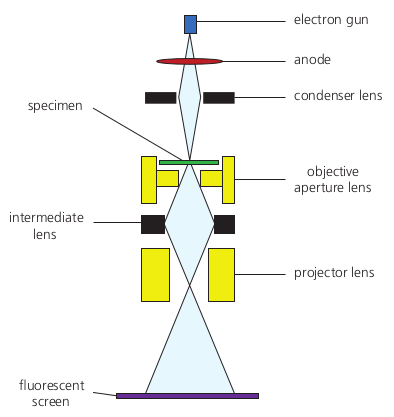
\includegraphics[width=8cm]{tem.png}\\
When an electron wave encounters the specimen it can either:
\begin{itemize}
\item Pass straight through the specimen without interacting
\item Get absorbed
\item Diffract
\end{itemize}
The electrons that pass through the specimen form the main beam, and a series of additional magnetic lenses direct and focus this beam onto a fluorescent screen. This creates an image when the electrons strike a florescent screen. The darker areas of the image represent the parts of the specimen that are thicker as more electrons are absorbed.\\
\\
The image detail can be improved by increasing the anode voltage of the electron gun.\\
\\
The image detail may reduce when travelling through the specimen as some electrons may have a loss of speed, causing the magnetic lenses to be unable to focus the electrons, a type of material dispersion.
\section{Scanning tunnelling microscope}
The STM has a very fine conducting probe, which is used to scan a small area of the surface of a conducting sample. The probe is positioned so that the tip of the probe is 1nm above the surface of the sample. The STM creates images using an effect known as quantum tunnelling, which allows some of the electrons in the tip of the probe or the sample to move across the 1nm gap, creating a tunnelling current between the sample and the probe. A small voltage is maintained between the tip of the probe and the sample to ensure that the electrons cross the gap in only one direction, from negative to positive.\\
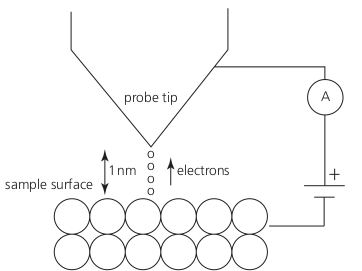
\includegraphics[width=5cm]{stm.png}\\
\\
Quantum tunnelling occurs because of the wave nature of electrons. Just as light can pass through a very thin metal film because the amplitude of the light is not reduced to zero by its passage through the film, matter waves can pass through an apparent barrier, such as an insulating air gap in a conducting circuit, if the gap is sufficiently narrow.\\
At room temperature the de Broglie wavelength of an electron in a metal is about 1nm, comparable to the gap between the sample surface and the probe tip, meaning there is a small probability that electrons can jump across the gap.\\
\\
A STM can be used in one of two ways:
\subsection{Method 1 - Constant height}
In this method the probe is kept at a constant height, so that only undulations in the surface of the sample affect the size of the gap. The smaller the gap, the more electrons move across the gap per second, increasing the current, which can then be measured.\\
The voltage between the surface and the probe tip must be kept constant, so the current at a given height is constant.\\
This has a vertical resolution of 0.001nm, much smaller than the smallest atom
\subsection{Method 2 - Constant current}
In this method the height of the probe is altered to keep the tunnelling current constant, and then variations in the vertical position of the probe can be used to image the surface of the sample.
\end{document}